\documentclass[14pt]{extbook}
\usepackage{multicol, enumerate, enumitem, hyperref, color, soul, setspace, parskip, fancyhdr} %General Packages
\usepackage{amssymb, amsthm, amsmath, bbm, latexsym, units, mathtools} %Math Packages
\everymath{\displaystyle} %All math in Display Style
% Packages with additional options
\usepackage[headsep=0.5cm,headheight=12pt, left=1 in,right= 1 in,top= 1 in,bottom= 1 in]{geometry}
\usepackage[usenames,dvipsnames]{xcolor}
\usepackage{dashrule}  % Package to use the command below to create lines between items
\newcommand{\litem}[1]{\item#1\hspace*{-1cm}\rule{\textwidth}{0.4pt}}
\pagestyle{fancy}
\lhead{Progress Quiz 4}
\chead{}
\rhead{Version C}
\lfoot{6286-1986}
\cfoot{}
\rfoot{Fall 2020}
\begin{document}

\begin{enumerate}
\litem{
First, find the equation of the line containing the two points below. Then, write the equation as $ y=mx+b $ and choose the intervals that contain $m$ and $b$.\[ (-2, -7) \text{ and } (7, 10) \]\begin{enumerate}[label=\Alph*.]
\item \( m \in [0.89, 3.89] \hspace*{3mm} b \in [2.76, 3.1] \)
\item \( m \in [-1.89, 1.11] \hspace*{3mm} b \in [23, 23.5] \)
\item \( m \in [0.89, 3.89] \hspace*{3mm} b \in [-5.32, -4.82] \)
\item \( m \in [0.89, 3.89] \hspace*{3mm} b \in [3.02, 3.32] \)
\item \( m \in [0.89, 3.89] \hspace*{3mm} b \in [-3.45, -3] \)

\end{enumerate} }
\litem{
Write the equation of the line in the graph below in Standard form $Ax+By=C$. Then, choose the intervals that contain $A, B, \text{ and } C$.
\begin{center}
    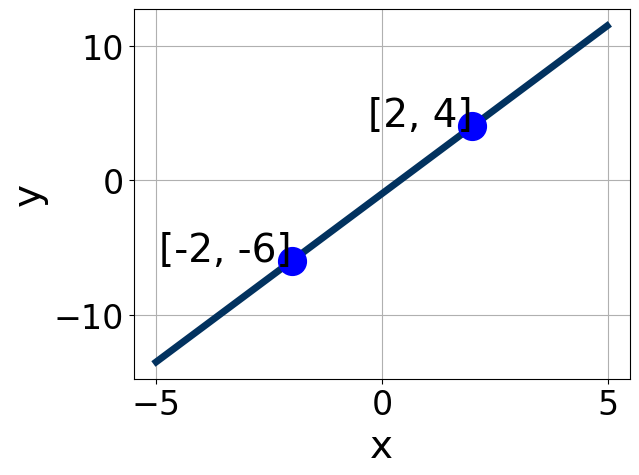
\includegraphics[width=0.5\textwidth]{../Figures/linearGraphToStandardCopyC.png}
\end{center}
\begin{enumerate}[label=\Alph*.]
\item \( A \in [1, 10], \hspace{3mm} B \in [1.27, 2.23], \text{ and } \hspace{3mm} C \in [-2.71, -1.47] \)
\item \( A \in [1, 10], \hspace{3mm} B \in [-2.99, -1.55], \text{ and } \hspace{3mm} C \in [1.38, 2.2] \)
\item \( A \in [-4.5, -0.5], \hspace{3mm} B \in [-1.25, -0.06], \text{ and } \hspace{3mm} C \in [0.82, 1.21] \)
\item \( A \in [-4.5, -0.5], \hspace{3mm} B \in [0.34, 1.84], \text{ and } \hspace{3mm} C \in [-1.69, -0.67] \)
\item \( A \in [-5, -3], \hspace{3mm} B \in [1.27, 2.23], \text{ and } \hspace{3mm} C \in [-2.71, -1.47] \)

\end{enumerate} }
\litem{
First, find the equation of the line containing the two points below. Then, write the equation as $ y=mx+b $ and choose the intervals that contain $m$ and $b$.\[ (-10, -8) \text{ and } (11, -2) \]\begin{enumerate}[label=\Alph*.]
\item \( m \in [0.24, 0.99] \hspace*{3mm} b \in [-5.35, -5.1] \)
\item \( m \in [0.24, 0.99] \hspace*{3mm} b \in [-13.11, -12.8] \)
\item \( m \in [-0.6, -0.22] \hspace*{3mm} b \in [0.99, 1.38] \)
\item \( m \in [0.24, 0.99] \hspace*{3mm} b \in [4.83, 5.41] \)
\item \( m \in [0.24, 0.99] \hspace*{3mm} b \in [1.97, 2.57] \)

\end{enumerate} }
\litem{
Solve the equation below. Then, choose the interval that contains the solution.\[ -19(7x + 9) = -8(13x + 10) \]\begin{enumerate}[label=\Alph*.]
\item \( x \in [-2.06, 0.94] \)
\item \( x \in [5.66, 11.66] \)
\item \( x \in [-10.66, -5.66] \)
\item \( x \in [-3.14, -2.14] \)
\item \( \text{There are no real solutions.} \)

\end{enumerate} }
\litem{
Solve the equation below. Then, choose the interval that contains the solution.\[ -12(9x + 19) = -3(-11x -15) \]\begin{enumerate}[label=\Alph*.]
\item \( x \in [-2.2, -1.91] \)
\item \( x \in [-2.77, -2.41] \)
\item \( x \in [-1.62, -1.12] \)
\item \( x \in [0.55, 2.03] \)
\item \( \text{There are no real solutions.} \)

\end{enumerate} }
\litem{
Solve the linear equation below. Then, choose the interval that contains the solution.\[ \frac{-3x + 8}{7} - \frac{-5x + 6}{6} = \frac{-3x -6}{2} \]\begin{enumerate}[label=\Alph*.]
\item \( x \in [-3.33, -2.39] \)
\item \( x \in [-4.62, -3.66] \)
\item \( x \in [-2.16, -0.87] \)
\item \( x \in [-1.16, 0.11] \)
\item \( \text{There are no real solutions.} \)

\end{enumerate} }
\litem{
Find the equation of the line described below. Write the linear equation as $ y=mx+b $ and choose the intervals that contain $m$ and $b$.\[ \text{Parallel to } 7 x - 8 y = 12 \text{ and passing through the point } (-2, 6). \]\begin{enumerate}[label=\Alph*.]
\item \( m \in [1.1, 1.8] \hspace*{3mm} b \in [7.63, 7.77] \)
\item \( m \in [0.03, 1.09] \hspace*{3mm} b \in [-7.83, -7.4] \)
\item \( m \in [-1.3, -0.76] \hspace*{3mm} b \in [4.2, 4.36] \)
\item \( m \in [0.03, 1.09] \hspace*{3mm} b \in [7.78, 8.1] \)
\item \( m \in [0.03, 1.09] \hspace*{3mm} b \in [7.63, 7.77] \)

\end{enumerate} }
\litem{
Find the equation of the line described below. Write the linear equation as $ y=mx+b $ and choose the intervals that contain $m$ and $b$.\[ \text{Perpendicular to } 8 x - 5 y = 5 \text{ and passing through the point } (5, 3). \]\begin{enumerate}[label=\Alph*.]
\item \( m \in [0.48, 1.26] \hspace*{3mm} b \in [-0.4, 1] \)
\item \( m \in [-1.55, -0.43] \hspace*{3mm} b \in [-2.7, -0.9] \)
\item \( m \in [-1.55, -0.43] \hspace*{3mm} b \in [-9.2, -5.8] \)
\item \( m \in [-3.08, -0.87] \hspace*{3mm} b \in [4.7, 8.2] \)
\item \( m \in [-1.55, -0.43] \hspace*{3mm} b \in [4.7, 8.2] \)

\end{enumerate} }
\litem{
Solve the linear equation below. Then, choose the interval that contains the solution.\[ \frac{-8x -4}{3} - \frac{-9x -7}{6} = \frac{-4x + 5}{4} \]\begin{enumerate}[label=\Alph*.]
\item \( x \in [-24.5, -21.5] \)
\item \( x \in [-10.5, -6.5] \)
\item \( x \in [-14, -10] \)
\item \( x \in [-2.72, 2.28] \)
\item \( \text{There are no real solutions.} \)

\end{enumerate} }
\litem{
Write the equation of the line in the graph below in Standard form $Ax+By=C$. Then, choose the intervals that contain $A, B, \text{ and } C$.
\begin{center}
    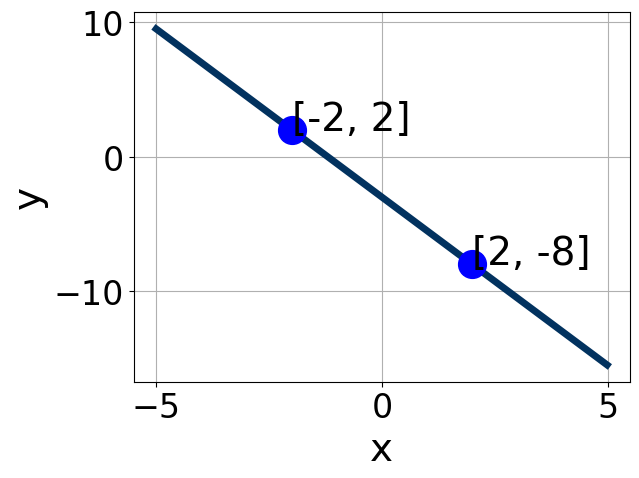
\includegraphics[width=0.5\textwidth]{../Figures/linearGraphToStandardC.png}
\end{center}
\begin{enumerate}[label=\Alph*.]
\item \( A \in [-6.1, -4.5], \hspace{3mm} B \in [-4.13, -2.59], \text{ and } \hspace{3mm} C \in [-3.32, -2.14] \)
\item \( A \in [-2.4, 3.4], \hspace{3mm} B \in [-1.75, -0.21], \text{ and } \hspace{3mm} C \in [-2.56, -0.54] \)
\item \( A \in [3.4, 7.3], \hspace{3mm} B \in [-4.13, -2.59], \text{ and } \hspace{3mm} C \in [-3.32, -2.14] \)
\item \( A \in [-2.4, 3.4], \hspace{3mm} B \in [0.67, 1.02], \text{ and } \hspace{3mm} C \in [-0.33, 1.41] \)
\item \( A \in [3.4, 7.3], \hspace{3mm} B \in [2.31, 3.82], \text{ and } \hspace{3mm} C \in [1.33, 3.51] \)

\end{enumerate} }
\end{enumerate}

\end{document}